Es  werden nun  anhand  der  Phasengangmethode sowohl  ein  PI-  wie auch  ein
PID-Regler f\"ur die in Abschnitt~\ref{subs:frequenzgang} ausgemessene Strecke
dimensioniert (siehe n\"achster Abschnitt f\"ur PID-Regler).

Folgende  Begriff   werden  dabei  h\"aufig   verwendet  und  sind   daher  in
Tabelle~\ref{tab:terms} \"ubersichtlich zusammengefasst.

\begin{longtable}{lp{60mm}}
    \toprule
    \endhead
    \endfoot
    \endlastfoot

    % CONTENT HERE ---------------------------------------------------------- %

    $H_s(j\omega)                                                                   $ &  \"Ubertragungsfunktion der Regelstrecke \\
    $A_s(j\omega)=|H_s(j\omega)|                                                    $ &  Amplitudengang der Regelstrecke \\
    $\varphi_s(j\omega)=arg(H_s(j\omega))                                           $ &  Phasengang der Regelstrecke \\
    $H_r(j\omega)                                                                   $ &  \"Ubertragungsfunktion des Reglers \\
    $A_r(j\omega)=|H_r(j\omega)|                                                    $ &  Amplitudengang des Reglers \\
    $\varphi_r(j\omega)=arg(H_r(j\omega))                                           $ &  Phasengang des Reglers \\
    $H_o(j\omega)=H_s \cdot H_r(j\omega)                                            $ &  \"Ubertragungsfunktion des offenen Regelkreises \\
    $A_o(j\omega)=|H_o(j\omega)|                                                    $ &  Amplitudengang des offenen Regelkreises \\
    $\varphi_o(j\omega)=arg(H_o(j\omega))=\varphi_s(j\omega)+\varphi_r(j\omega)     $ &  Phasengang des offenen Regelkreises \\
    $H_{rpid}= K_{rk}\Big[ \frac{(1+sT_{nk})(1+sT_{vk})}{sT_{nk}}\Big]              $ & \"Ubertragungsfunktion des PID-Reglers \\
    $H_{rpi} = K_{rk}\Big[ 1 + \frac{1}{sT_{nk}} \Big]                              $ & \"Ubertragungsfunktion des PI-Reglers \\

    \bottomrule
    \caption{Die wichtigsten Begriffsdefinitionen}
    \label{tab:terms}
\end{longtable}


\subsubsection*{Ziel}
Das  Ziel ist  die  Bestimmung  der Parameter  $K_{rk}$  und  $T_{nk}$ in  der
Gleichung:

\begin{equation} \label{eq:pi:target}
    H_{rpi} = K_{rk} \cdot \biggl[ 1 + \frac{1}{s \cdot T_{nk}} \biggr]
\end{equation}


\subsubsection{Bestimmung der Reglerfrequenz $\omega_{pi}$}

Zuerst wird im Phasengang der Strecke die Frequenz $\omega_{pi}$ bestimmt, f\"ur
welche die Phase der Strecke $-90\degree$ betr\"agt\footnotemark[1].

\begin{equation} \label{eq:pi:phi_s}
    \varphi_s(\omega_{pi}) = -90 \degree
\end{equation}

\footnotetext[1]{%
    Der  Winkel  stellt  keinen   endg\"ultigen  Wert  dar. Dieser  wurde  von
    Jakob  Zellweger  fixiert, um  eine  grafische  Evaluation \"uberhaupt  zu
    erm\"oglichen. Durch Anpassung dieses Wertes kann je nach Regelstrecke das
    Regelverhalten weiter optimiert werden.
}

\begin{figure}[h! width=\pagewidth]
    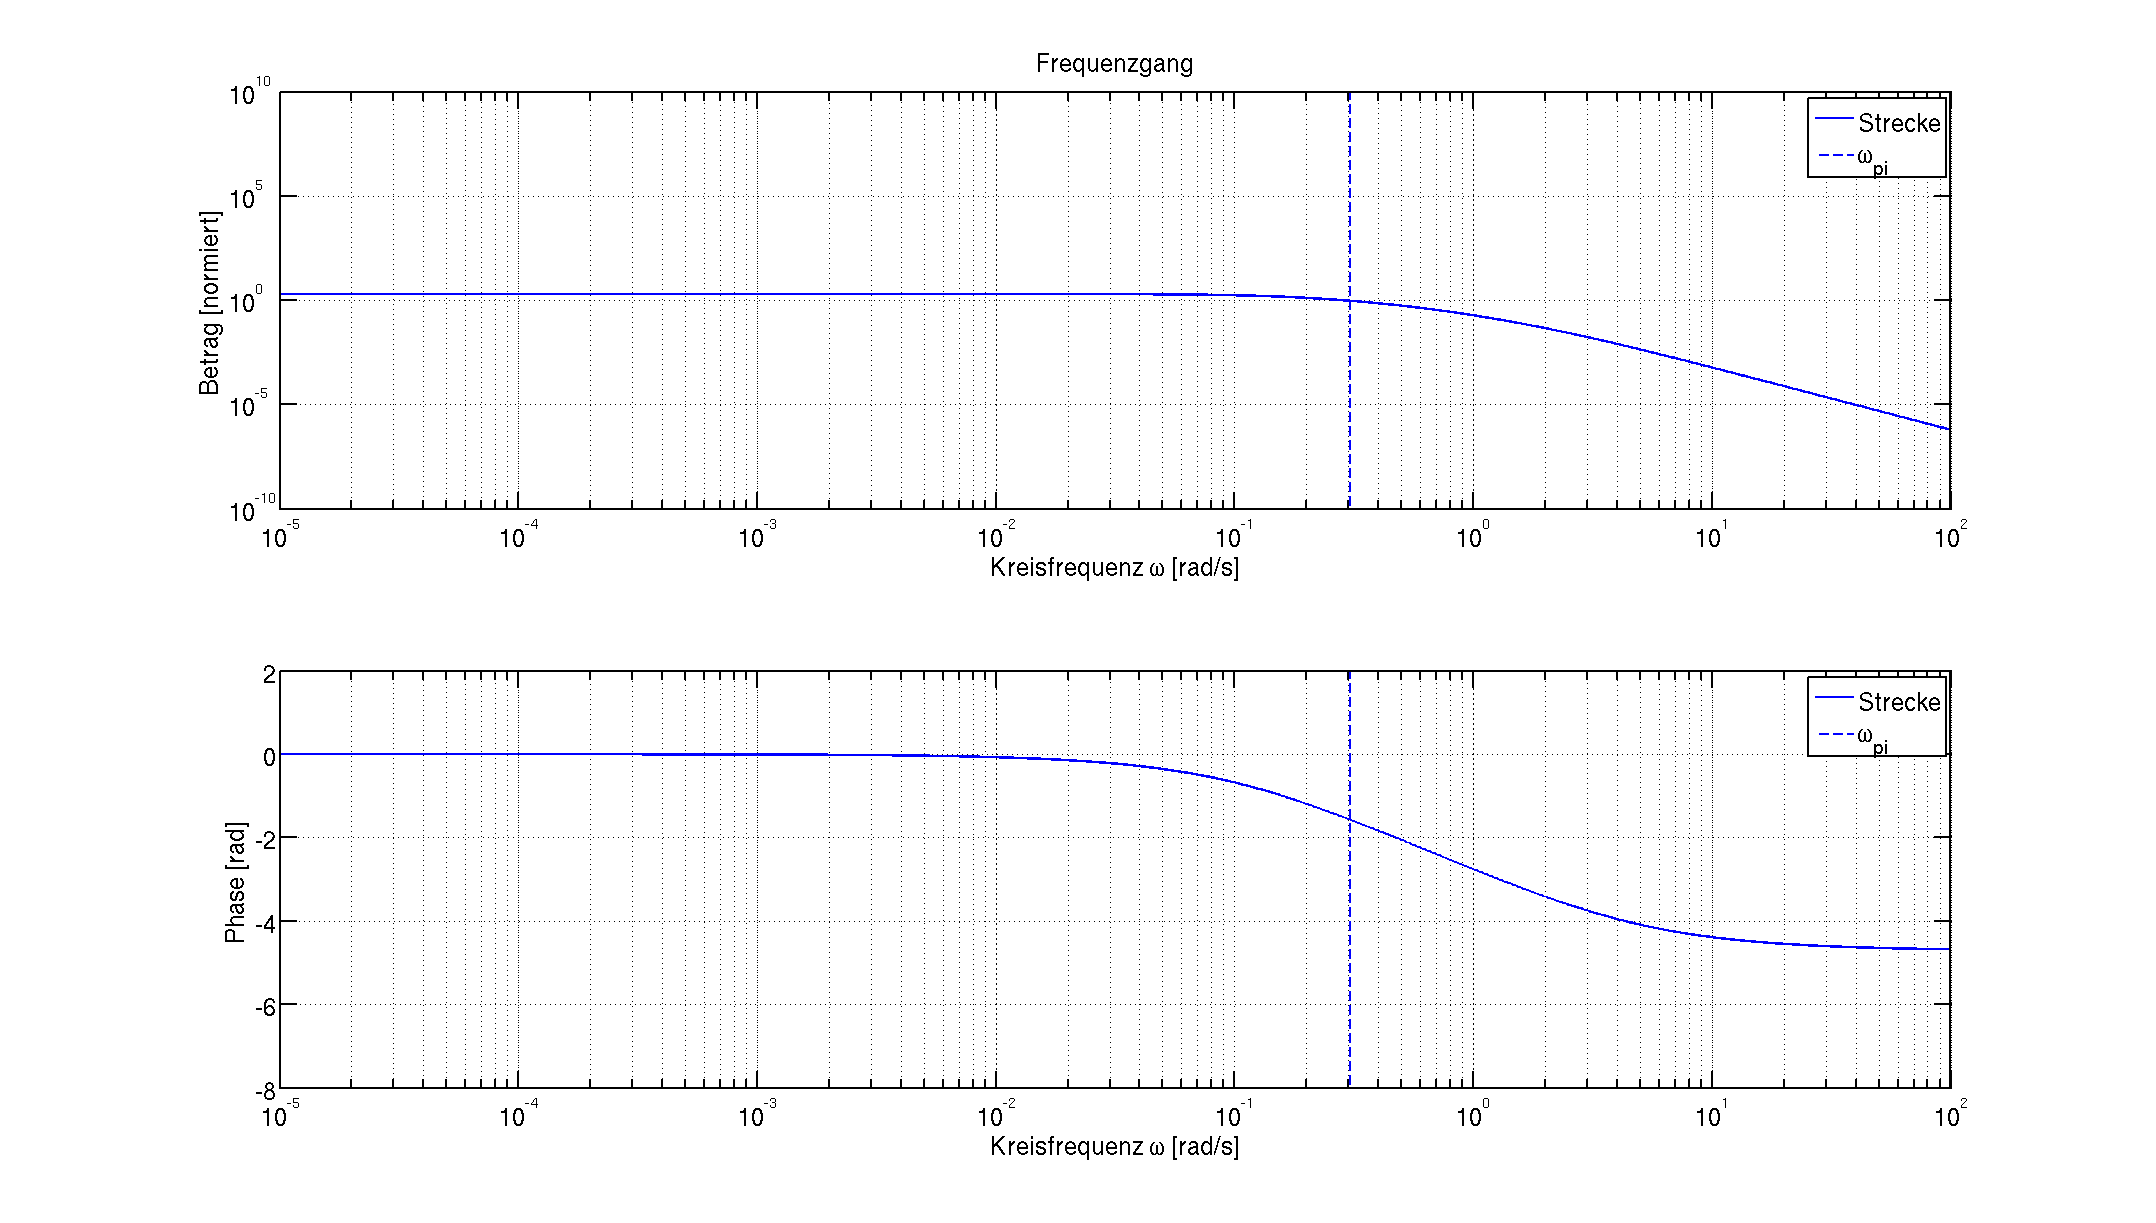
\includegraphics[width=\textwidth]{images/piStreckeOmegaPI.png}
    \caption{%
        $\omega_{pi}$ eingetragen (vertikale gestrichelte Linie).
    }
    \label{fig:pi:omega_pi}
\end{figure}

Wie    man   aus    Abbildung~\ref{fig:pi:omega_pi}   ablesen    kann,   liegt
dieser   Wert  f\"ur   $\omega_{pi}$  in   unserem  Beispiel   bei  ungef\"ahr
$\SI{0.3}{\per\second}$. Die Kontrollrechnung mittels Matlab ergibt:

\begin{equation} \label{eq:pi:omega_pi}
    \omega_{pi} = \SI{0.3039}{\per\second}
\end{equation}


\subsubsection{Bestimmung von $T_{nk}$}
Damit kann nun $T_{nk}$ direkt bestimmt werden\footnotemark[2]:

\begin{equation} \label{eq:pi:omega_pi}
    T_{nk} = \frac{1}{\omega_{pi}} = \frac{1}{\SI{0.3039}{\per\second}} = \SI{3.2902}{\second}
\end{equation}

\footnotetext[2]{%
    Um die  Akkumulation von Ungenauigkeiten  zu minimieren werden  bei diesen
    Berechnungen  die  genauen  Werte  aus  Matlab  verwendet  und  nicht  die
    gerundeten  Zwischenresultate,  was  zu   Abweichungen  zu  den  von  Hand
    berechneten Ergebnissen f\"uhren kann.
}


\subsubsection{Bestimmung der Durchtrittsfrequenz $\omega_d$}

Als N\"achstes  soll die Durchtrittsfrequenz $\omega_d$  bestimmt werden. Dazu
wird  der  f\"ur  $T_{nk}$  erhaltene  Wert  in  Gleichung~\ref{eq:pi:target}
eingesetzt. Da $K_{rk}$ noch unbekannt ist, wird vorerst $K_{rk} = 1$ gesetzt.

\begin{gather} \label{eq:pi:target}
    \begin{split}
        H_{rpi} & = K_{rk} \cdot \biggl[ 1 + \frac{1}{s \cdot T_{nk}} \biggr] \\
                & = 1      \cdot \biggl[ 1 + \frac{1}{s \cdot \SI{3.2902}{\second}} \biggr]
    \end{split}
\end{gather}

Daraus   kann   nun   der   Frequenzgang   des   \emph{offenen   Regelkreises}
(\"Ubertragungsfunktion $H_o$,  Amplitudengang $A_o$,  Phasengang $\varphi_o$)
bestimmt werden.

\begin{gather} \label{eq:pi:h_open}
    \begin{split}
        H_o (s) & = H_{rpi} (s) \cdot H_s (s) \\
            & = \Biggl(
                    K_{rk} \cdot \biggl[ 1 + \frac{1}{s \cdot T_{nk}} \biggr]
                \Biggr)
                \cdot
                K_s
                \cdot
                \Biggl(
                        \frac{1}{1 + s \cdot T_1}
                  \cdot \frac{1}{1 + s \cdot T_2}
                  \cdot \frac{1}{1 + s \cdot T_2}
                \Biggr) \\
            & = \Biggl(
                    1 \cdot \biggl[ 1 + \frac{1}{s \cdot \SI{3.2902}{\second}} \biggr]
                \Biggr)
                \cdot
                2
                \cdot
                \Biggl(
                          \frac{1}{1 + s \cdot \SI{0.4134}{\second}}
                    \cdot \frac{1}{1 + s \cdot \SI{1.4894}{\second}}
                    \cdot \frac{1}{1 + s \cdot \SI{5.3655}{\second}}
                \Biggr)
    \end{split}
\end{gather}


Wobei der Amplitudengang den Betragsverlauf und der Phasengang den Verlauf des
Arguments dieser \"Ubertragungsfunktion repr\"asentieren:

\begin{equation}
    \begin{split} \label{eq:pi:a_o_phi_o}
        A_o(j\omega)       & = |H_o(j\omega)| \\
        \varphi_o(j\omega) & = arg(H_o(j\omega))
    \end{split}
\end{equation}

Von besonderem  Interesse ist  hier der Phasengang. Wie  Anfangs spezifiziert,
soll  ein maximals  \"Uberschwingen von  ca. $16.3\%$ angestrebt  werden. Dazu
muss  gem\"ass  Tabelle~\ref{tab:phi_s}   die  Durchtrittsfrequenz  $\omega_d$
gefunden   werden,  an   welcher  der   offene  Regelkreis   eine  Phase   von
$-128.5\degree$ aufweist.

\begin{longtable}{llll}
    \toprule
    \endhead
    \endfoot
    \endlastfoot

    % CONTENT HERE ---------------------------------------------------------- %

    \"Uberschwingen & 0\%              & 16.3\%           & 23.3\% \\
    $\varphi_s$        & $-103.7 \degree$ & $-128.5 \degree$ & $-135 \degree$ \\

    \bottomrule
    \caption{Werte f\"ur $\varphi_s$}
    \label{tab:phi_s}
\end{longtable}

\begin{figure}[h! width=\pagewidth]
    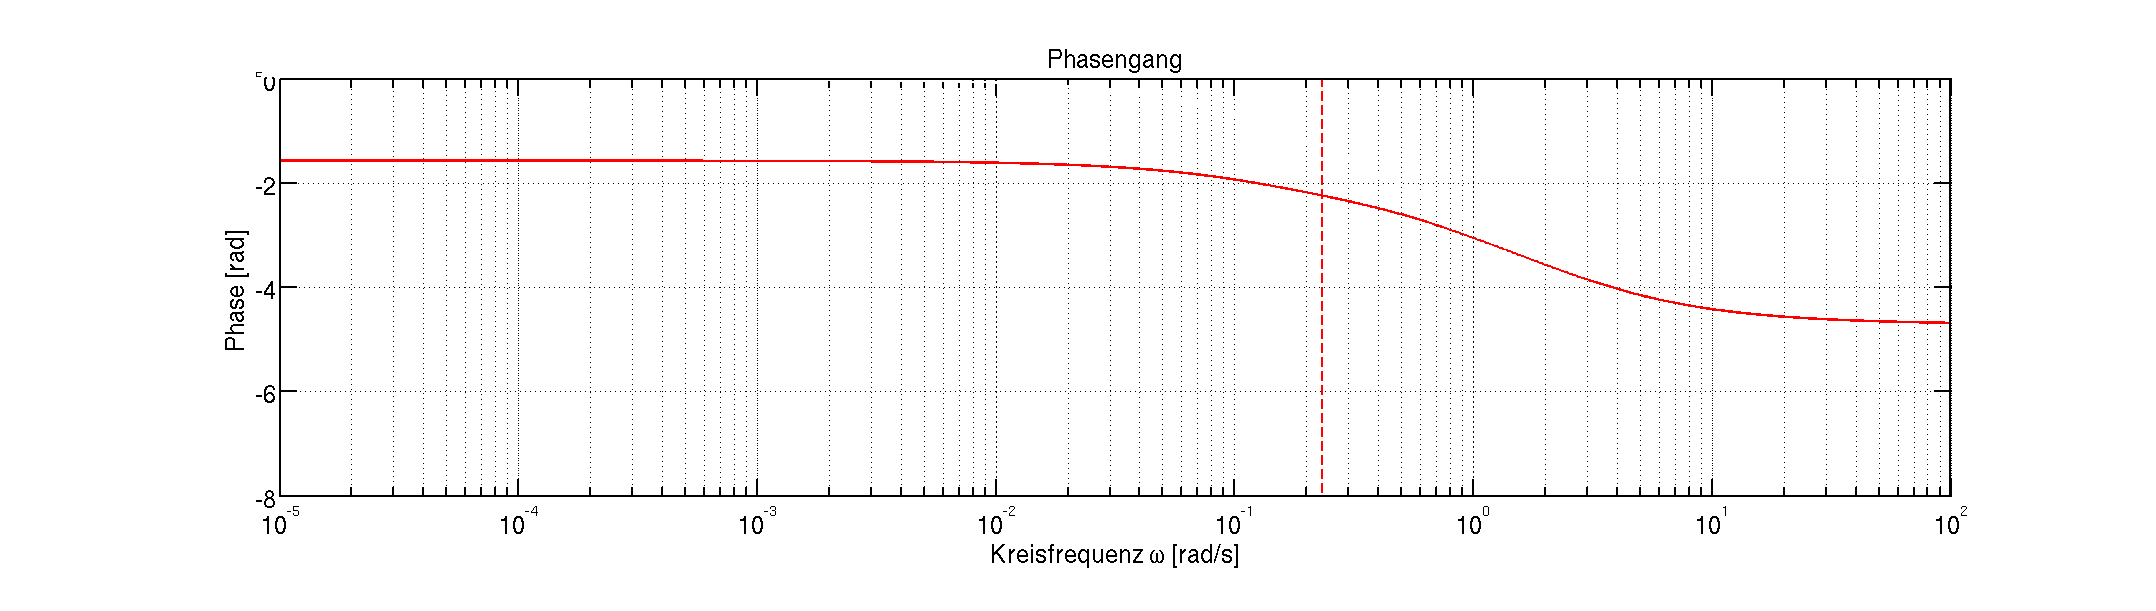
\includegraphics[width=\textwidth]{images/piOffenerRegelkreisPhasengang.png}
    \caption{%
        Phasengang   $\varphi_o(j\omega)$   des   offenen   Regelkreises   mit
        eingetragener Durchtrittsfrequenz $\omega_{d}$ (vertikale gestrichelte
        Linie). Wie man verifizieren kann, weist der offene Regelkreis unseres
        Beispiels bei dieser Kreisfrequenz  eine Phase von $-128.5\degree$ auf
        (etwa $\SI{-2.24}{\radian}$).
    }
    \label{fig:pi:omega_d}
\end{figure}

Dies ergibt:
\begin{equation} \label{eq:pi:omega_d}
    \omega_d = \SI{0.2329}{\per\second}
\end{equation}


\subsubsection{Bestimmung der Reglerverst\"arkung $K_{rk}$}

In  einem  letzten  Schritt  wird  nun  die  Durchtrittsfrequenz  benutzt,  um
die  ben\"otigte Verst\"arkung  $K_{rk}$ des  Reglers zu  bestimmen. Dazu wird
$\omega_d$  in  Gleichung~\ref{eq:pi:h_open}  eingesetzt  und  $|H_o(j\omega)|
=   1$  gesetzt   (Durchtrittsfrequenz: Frequenz,   bei   der  die   Amplitude
$\SI{0}{\decibel} = 1$ ist).

\begin{gather} \label{eq:pi:A_o_set_to_one}
    \begin{split}
        A_o & = | H_o (j\omega_d) | \\
            & = \abs*{
                    \bigg(
                        K_{rk} \cdot \biggl[ 1 + \frac{1}{j \cdot \omega_d \cdot T_{nk}} \biggr]
                    \bigg)
                    \cdot
                    K_s
                    \cdot
                    \bigg(
                            \frac{1}{1 + j \cdot \omega_d \cdot T_1}
                      \cdot \frac{1}{1 + j \cdot \omega_d \cdot T_2}
                      \cdot \frac{1}{1 + j \cdot \omega_d \cdot T_2}
                      \bigg)} \\
              & = 1
    \end{split}
\end{gather}

Mit den Werten
\begin{equation} \label{eq:pi:values}
    \begin{split}
        K_s      & = 2                    \\
        T_{nk}   & = \SI{3.2902}{\second} \\
        T_1      & = \SI{0.4134}{\second} \\
        T_2      & = \SI{1.4894}{\second} \\
        T_3      & = \SI{5.3655}{\second} \\
        \omega_d & = \SI{0.2329}{\radian\per\second}
    \end{split}
\end{equation}

l\"ost  man Gleichung  \ref{eq:pi:A_o_set_to_one}  nun nach  $K_{rk}$ auf  und
erh\"alt:

\begin{equation} \label{eq:pi:k_rk_result}
    K_{rk} = 0.517577
\end{equation}


\subsubsection{Resultat}

Somit ist der PI-Regler vollst\"andig bestimmt und hat folgende Form:

\begin{equation} \label{eq:pi:result}
    H_{rpi} = 0.518 \cdot \biggl[ 1 + \frac{1}{s \cdot \SI{3.29}{\second}} \biggr]
\end{equation}

Zum Vergleich das Bode-Diagramm mit allen relevanten Kurven und Werten:
\begin{figure}[h! width=\pagewidth]
    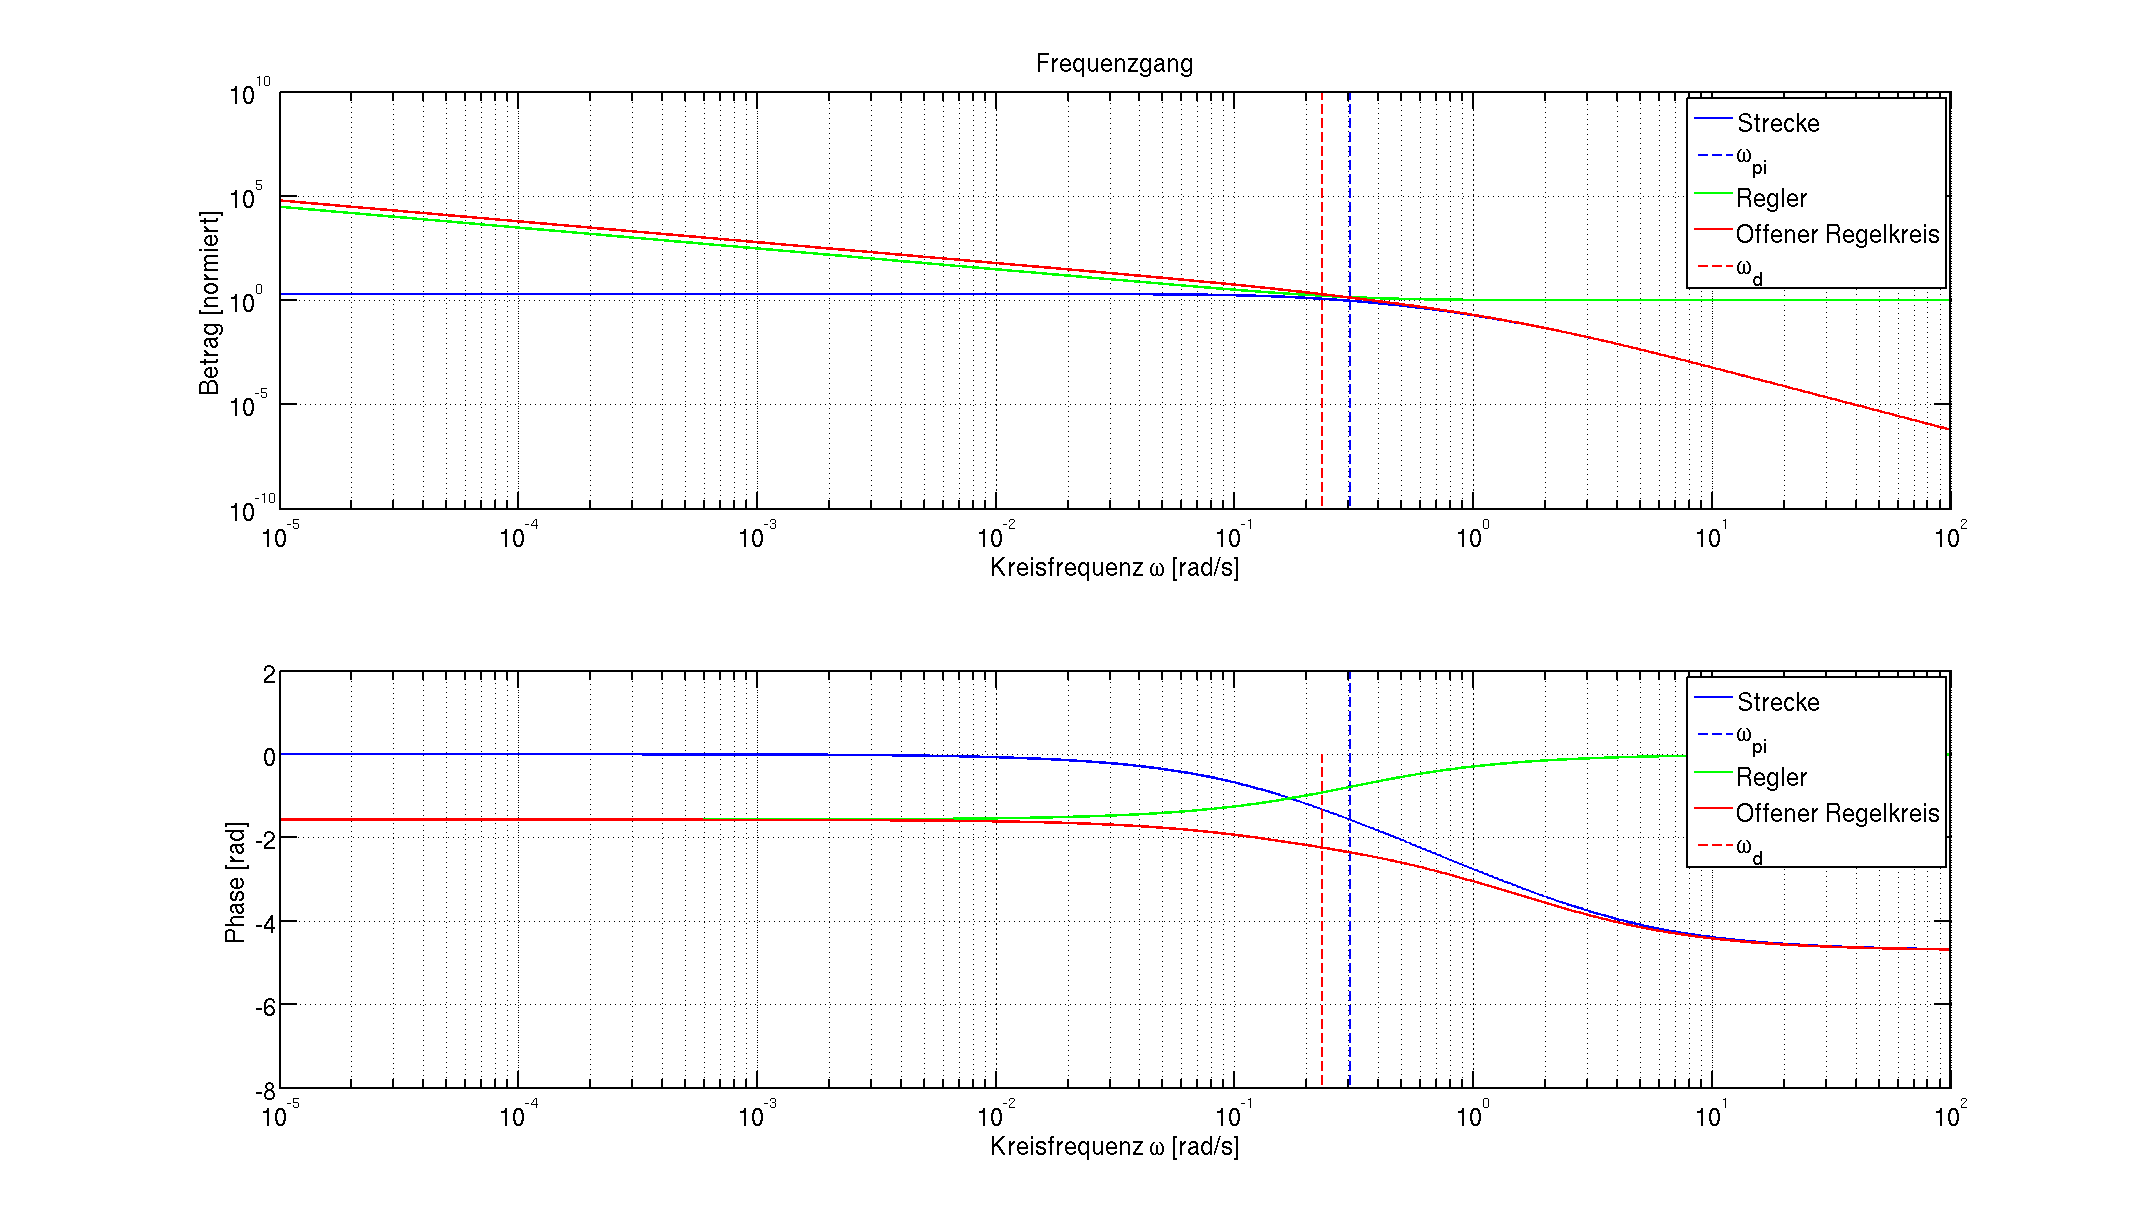
\includegraphics[width=\textwidth]{images/piBode.png}
    \caption{%
        Frequenzgang des Reglers (gr\"un), der  Strecke (blau) und des offenen
        Regelkreises (rot).
    }
    \label{fig:pi:all}
\end{figure}
\todo{Fix vertical line $\omega_d$}
